%%%%%%%%%%%%%%%%%%%%%%%%%%%%%%%%%%%%%%%%%
% Short Sectioned Assignment
% LaTeX Template
% Version 1.0 (5/5/12)
%
% This template has been downloaded from:
% http://www.LaTeXTemplates.com
%
% Original author:
% Frits Wenneker (http://www.howtotex.com)
%
% License:
% CC BY-NC-SA 3.0 (http://creativecommons.org/licenses/by-nc-sa/3.0/)
%
%%%%%%%%%%%%%%%%%%%%%%%%%%%%%%%%%%%%%%%%%

%----------------------------------------------------------------------------------------
%	PACKAGES AND OTHER DOCUMENT CONFIGURATIONS
%----------------------------------------------------------------------------------------

\documentclass[paper=a4, fontsize=12pt]{scrartcl} % A4 paper and 11pt font size
\usepackage{multirow}
\usepackage[T1]{fontenc} % Use 8-bit encoding that has 256 glyphs
\usepackage{fourier} % Use the Adobe Utopia font for the document - comment this line to return to the LaTeX default
\usepackage[english]{babel} % English language/hyphenation
\usepackage{amsmath,amsfonts,amsthm} % Math packages
\usepackage{booktabs}
\usepackage{sectsty} % Allows customizing section commands
\allsectionsfont{\centering \normalfont\scshape} % Make all sections centered, the default font and small caps
\usepackage{rotating}
\usepackage{graphicx}

\usepackage[a4paper,lmargin=2.5 cm,rmargin=2 cm,tmargin=2 cm,bmargin=2 cm]{geometry}

\usepackage{fancyhdr} % Custom headers and footers
\pagestyle{fancyplain} % Makes all pages in the document conform to the custom headers and footers
\fancyhead{} % No page header - if you want one, create it in the same way as the footers below
\fancyfoot[L]{} % Empty left footer
\fancyfoot[C]{} % Empty center footer
\fancyfoot[C]{\thepage} % Page numbering for right footer
\renewcommand{\headrulewidth}{0pt} % Remove header underlines
\renewcommand{\footrulewidth}{0pt} % Remove footer underlines
\setlength{\headheight}{13.6pt} % Customize the height of the header

\usepackage{chngcntr}
%\numberwithin{equation}{section} % Number equations within sections (i.e. 1.1, 1.2, 2.1, 2.2 instead of 1, 2, 3, 4)
%\numberwithin{figure}{section} % Number figures within sections (i.e. 1.1, 1.2, 2.1, 2.2 instead of 1, 2, 3, 4)
%\counterwithout{figure}{section}
%\numberwithin{table}{section} % Number tables within sections (i.e. 1.1, 1.2, 2.1, 2.2 instead of 1, 2, 3, 4)

%\setlength\parindent{0pt} % Removes all indentation from paragraphs - comment this line for an assignment with lots of text
\setlength\parindent{24pt}

\usepackage{amsmath}
\usepackage{float} % To firce the location of figure
\usepackage{subfigure} %For side-by-side figures
\usepackage{lettrine}
%\usepackage{lipsum}
\usepackage{epstopdf} %To read *.eps Files
\usepackage{listings} % To include source codes in LATEX document
\usepackage{mathrsfs} % To include script fonts. use \mathscr{}
\usepackage{courier} % To write in courier fornt
\usepackage{mathtools} % For mat symbols
\usepackage{xfrac} % For \sfrac{}{}
\usepackage{listings}
%----------------------------------------------------------------------------------------
%	TITLE SECTION
%----------------------------------------------------------------------------------------

\newcommand{\horrule}[1]{\rule{\linewidth}{#1}} % Create horizontal rule command with 1 argument of height

\title{	
\normalfont \normalsize 
\textsc{Wright State University\\ Department of Mechanical and Materials Engineering} \\ [25pt] % Your university, school and/or department name(s)
\horrule{0.5pt} \\[0.4cm] % Thin top horizontal rule
\huge ME 7060 - Structural Reliability \\ % The assignment title
\Large Project Proposal: Reliability Analysis of an AGM-86 ALCM Wing's Natural Frequencies
\horrule{2pt} \\[0.5cm] % Thick bottom horizontal rule
}

\author{Daniel Clark and Admir Makas} % Your name

\date{\normalsize March 2, 2015} % Today's date or a custom date

\begin{document}

\maketitle % Print the title

%----------------------------------------------------------------------------------------
%	Introduction
%----------------------------------------------------------------------------------------
\section*{Introduction}
Reliability of engineering systems has received great deal of scrutiny since the turn of the 20th century, this is mainly due to the industrial revolution. For the first time in human history products were mass produced on a large scale in order to meet the demand of the consumer public. At this time it was quickly realized that engineering and manufacturing process controls were instrumental in ensuring robust design and proper system function throughout the product lifecycle. The aforementioned process controls were built mainly with the use of stochastic methodologies, which aimed to increase the reliability of products by reducing the probability of failure. At the onset of the industrial revolution, material fatigue quickly became a critical parameter, which controlled the robustness and reliability of many manufactured products. Fatigue is inherently a random variable, which depends on many input parameters that include but are not limited to load, material, and dimensional variations. As a result, great deal of emphasis was placed on accurate fatigue predictions using statistical methods. These methods can be used in conjunction with testing and simulations to realize a robust and reliable design.

Many engineering fields are affected by fatigue and aerospace industry is no exception. The design of an aircraft wing for example is strongly influenced by its fatigue properties. Additionally, wings are typically dynamically loaded which adds another level of complexity to the fatigue estimation of the wing system. One critical aspect of proper fatigue quantification is to accurate prediction of the natural frequencies and mode shapes that govern the wing oscillation characteristics. As is the case with fatigue, frequency response of the wing is a random variable that depends on the initial material and dimensional inputs, which themselves are randomly distributed. 

The goal of the proposed project is to identify critical parameters which govern the modal response of the wing and use estimated random distributions of the inputs to obtain a distribution for the resultant natural frequencies. The first five modes of the AGM-86 ALCM cruise missile, Fig. \ref{fig:cruiseMissile}, will be investigated in detail. Calculations will be carried out using finite element (FE) simulations, which will incorporate input variability to obtain a distribution of results. The FE results will be validated based on experimental results. Obtaining robust confidence intervals for the natural frequencies will ensure more accuracy for fatigue estimations that may be done at a later time. 
%
\begin{figure}[H]
	\centering
	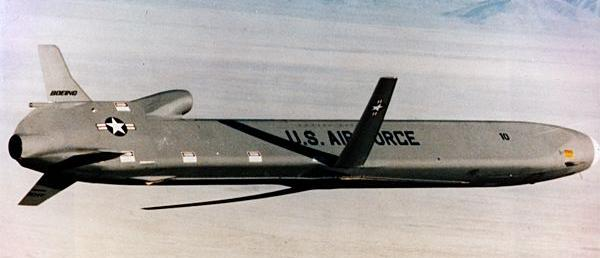
\includegraphics[height = 4.0cm]{Pictures/agm-86c.jpg}
	\caption{\textbf{AGM-86 ALCM.} Photo of the AGM-86 ALCM is an American subsonic air-launched cruise missile built by Boeing.}
	\label{fig:cruiseMissile}
\end{figure}
%
%----------------------------------------------------------------------------------------
%	Wing Description
%----------------------------------------------------------------------------------------
\section*{Wing Description}
The AGM-86's wings are critical to maintain stability at Mach 0.73 and accuracy over its 1,500+ mile operational range. An enlarged photo of the wings position on the missile is in Fig. \ref{fig:cruiseMissile_wing}. The wing dimensions are approximately: 1671.5 mm long, 180 mm wide at the tip, 330 mm wide at the base, with a 30 degree offset from the vertical. The airfoil shape has an approximate chord thickness of 18.30 mm and a blunted trailing edge. It is also assumed the wing is constructed from aluminum.
%
\begin{figure}[H]
	\centering
	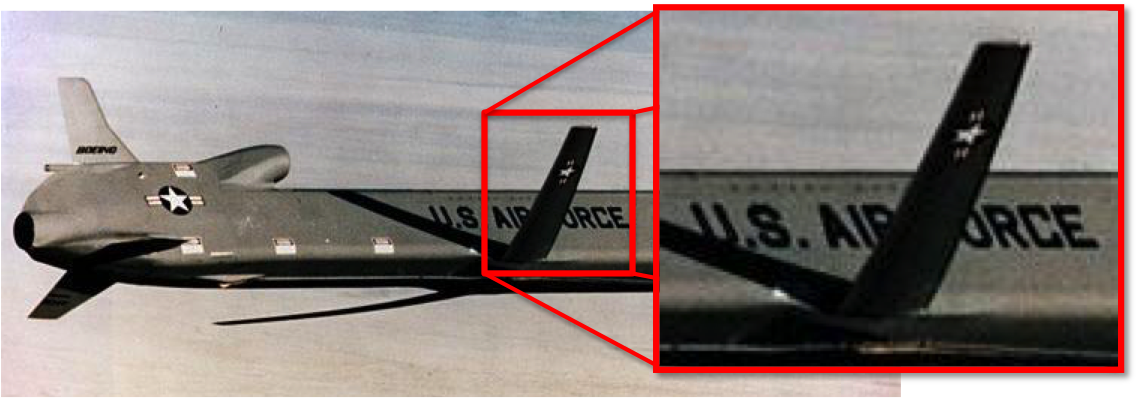
\includegraphics[height = 4.0cm]{Pictures/wing.png}
	\caption{\textbf{Stabilizing Wing.} Enlarged view of the AGM-86 ALCM's right wing.} 
	\label{fig:cruiseMissile_wing}
\end{figure}
%
Two finite element model were built to ensure the wing was accurately represented, Fig. \ref{fig:cruiseMissile_FEMS}. The first model was constructed utilizing beam and truss elements of various thicknesses in NX Nastran with cantilever boundary conditions (BC). The second model was also constructed in NX Nastran with similar BC's, but utilized shell elements. When compared computationally, the second model takes an additional five seconds to run. However, the additional time does not imply more accurate results when compared to the experiment. The wire model was demonstrated to be more accurate and quicker. Therefore, it has been selected for reliability assessment.
%
\begin{figure}[H]
	\centering
	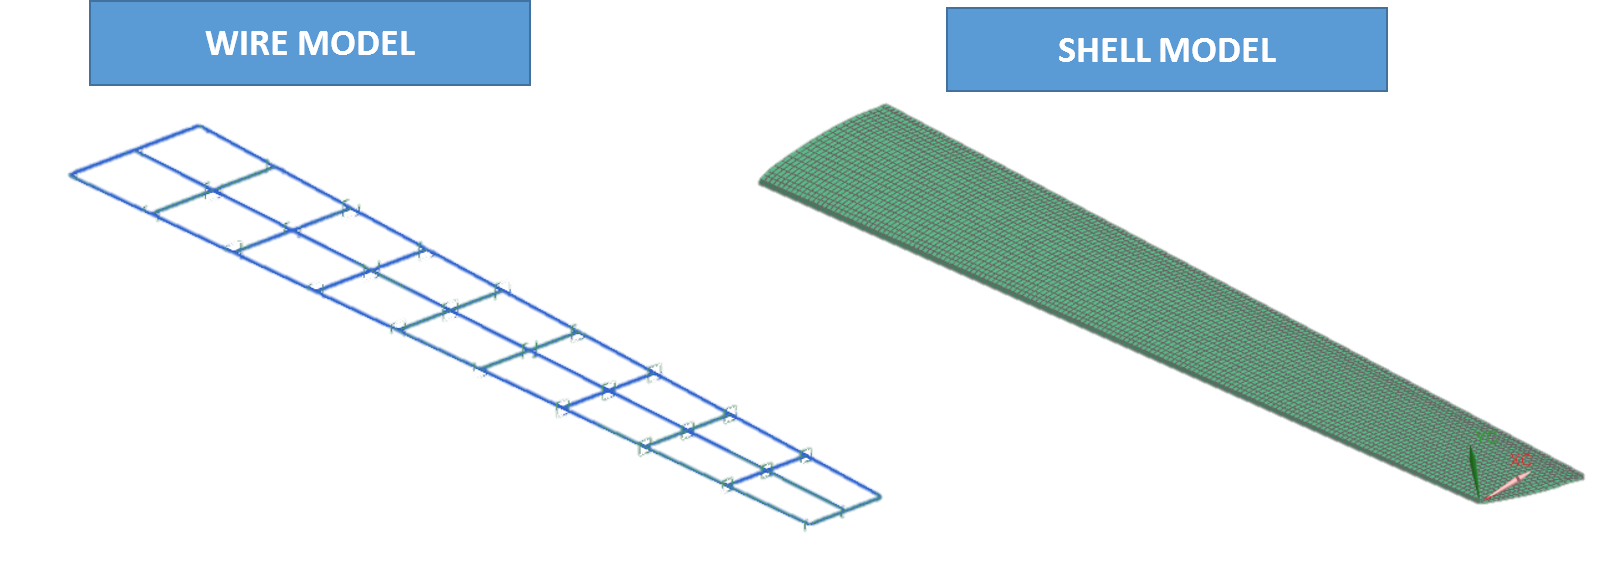
\includegraphics[height = 5.0cm]{Pictures/FEMs.png}
	\caption{\textbf{Finite Element Models.} A) Beam and truss configuration of the FEM B) Shell element FEM.} 
	\label{fig:cruiseMissile_FEMS}
\end{figure}
%
The experimental setup is shown in Fig. \ref{fig:cruiseMissile_setup}. The cruise missile wing is bolted/clamped into a test stand placed onto the ground. Some of the experimental data and FEM results of the wire model are in Table \ref{table:ERROR} and Fig. \ref{fig:cruiseMissile_FRF}.
%
\begin{figure}[H]
	\centering
	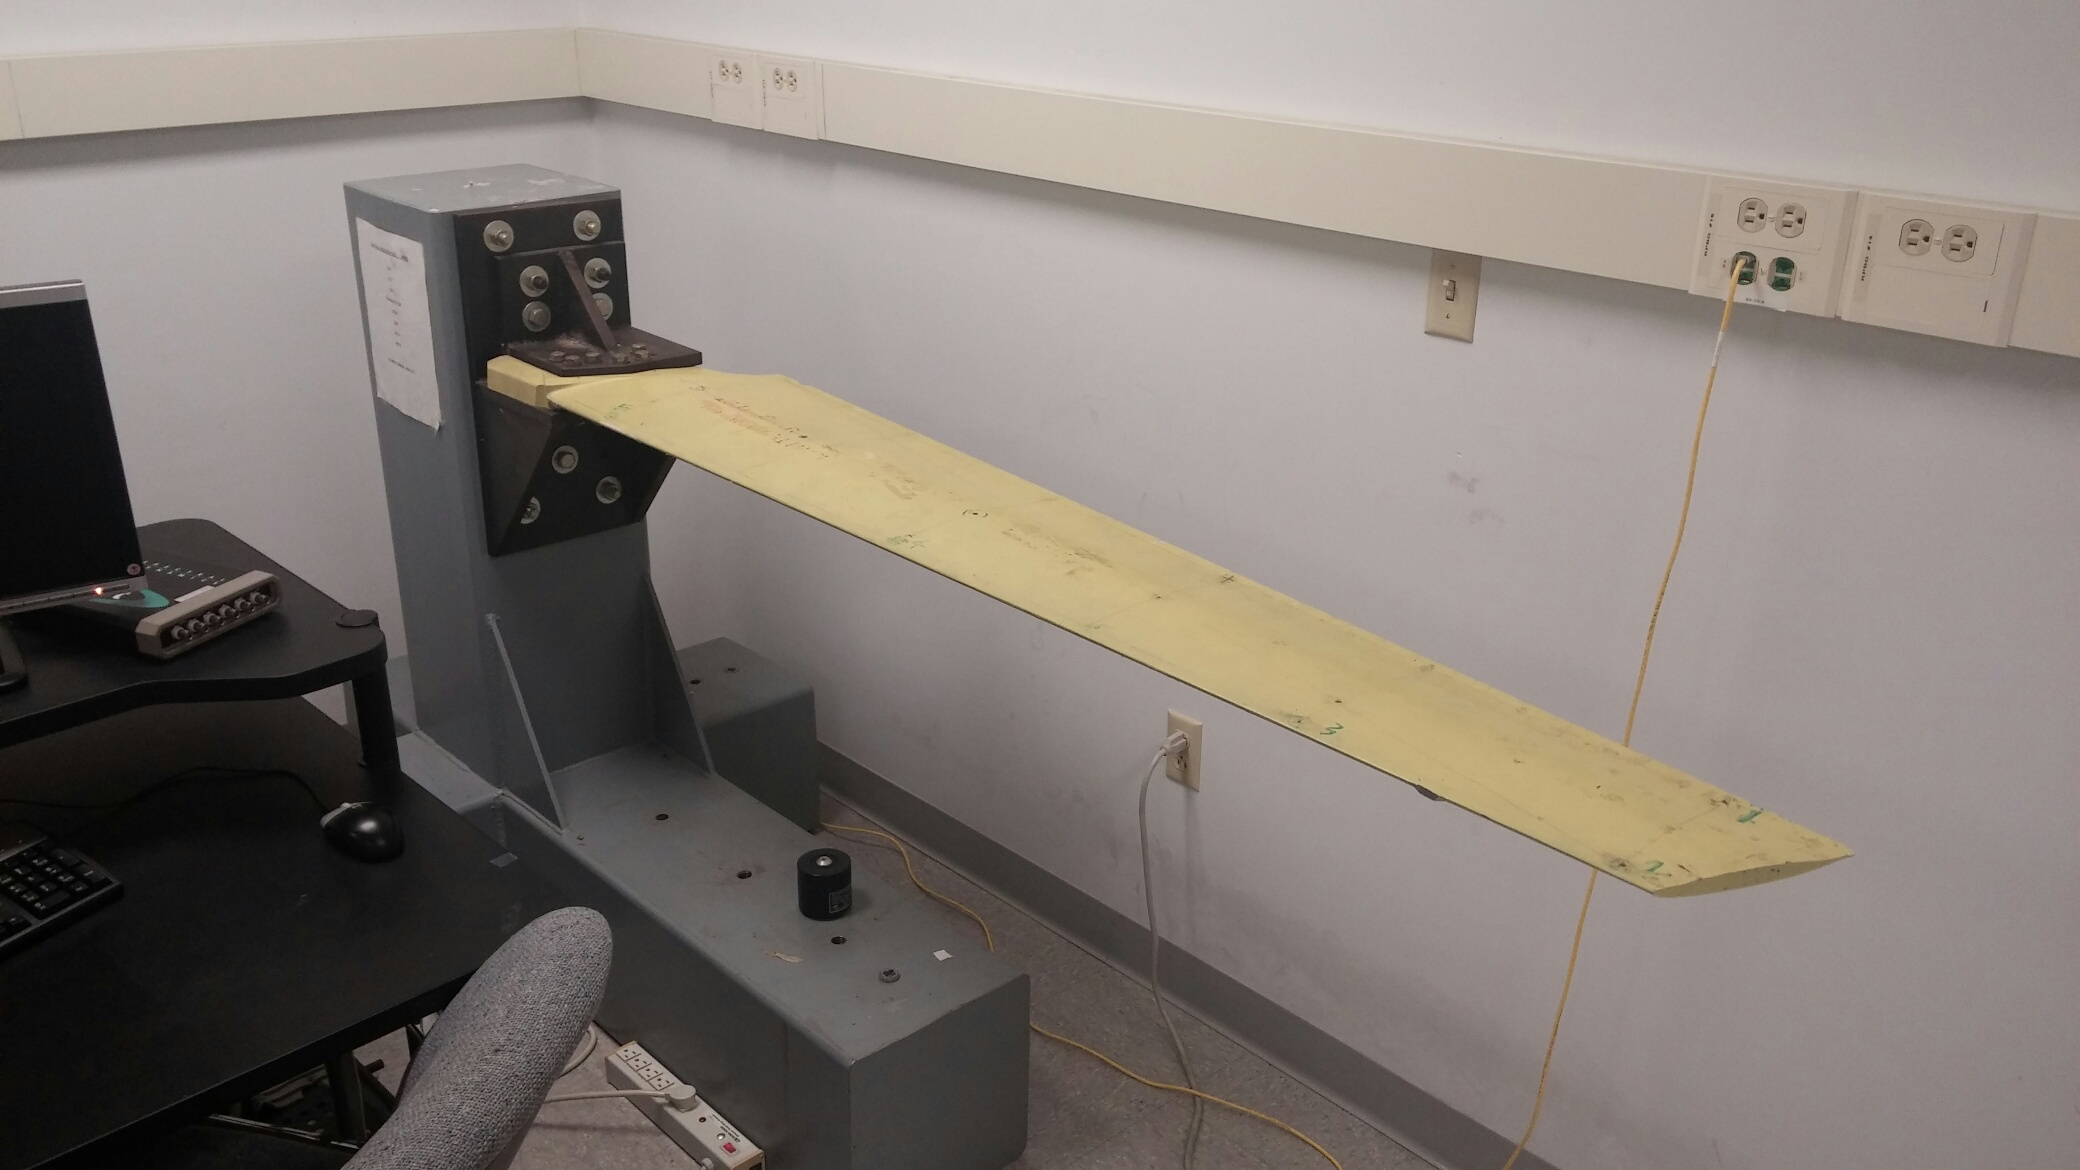
\includegraphics[height = 7.0cm]{Pictures/expSetUp.jpg}
	\caption{\textbf{The Experimental Setup.} Cruise missile wing attached to experimental fixture. } 
	\label{fig:cruiseMissile_setup}
\end{figure}
%
%----------------------------------------------------------------------------------------
%	Objective
%----------------------------------------------------------------------------------------
\section*{Objective}
The objective of this study is to determine the distributions of the first 5 natural frequencies utilizing the experimental setup in Fig. \ref{fig:cruiseMissile_setup} to determine the distributions of the input parameters. The experiment will also be used to Validate and Verify the FEM results. The parameters and distributions considered for the FEM are in Table \ref{table:RV}. 
%
\begin{table}[H]
\centering
\caption{Random Variables.}
\begin{tabular}{| c | c | c | c |}
\hline
		Variable & Abbreviation & Distribution & Determined \\ \hline
		\hline
		Young's Modulus & E & Lognormal & Experimentally \\ \hline
		Damping Ratio & $\zeta$ &  Lognormal & Experimentally  \\ \hline
		Poisson's Ratio & $\mu$ & Lognormal & Experimentally \\ \hline
		Thickness  & t & Normal  & Assumed \\ \hline
		Length & L  &  Normal  & Assumed \\ \hline
		Chord  & C & Normal  & Assumed \\ \hline
\end{tabular}
\label{table:RV}
\end{table}
%
The following parameter distributions can be verified via experiments in the dynamics lab: Young's Modulus, Poisson's Ratio and Damping Ratio. For the Young's Modulus there is a possibility to evaluate a confidence interval of the mean on the experiments conducted the lab. A confidence interval can also be determined for the Poisson's ratio. The mean of the Dampening ratio can also be evaluated experimentally by estimating the by back calculating from the measured mode shapes. The Thickness, Length and Chord will all be assumed to be Normally distributed due to manufacturing tolerances. The working mean or the deterministic wire FEM is compared to the experimental results in Table \ref{table:ERROR} and the frequency response function of the wing is shown in Fig. \ref{fig:cruiseMissile_FRF}.
%
\begin{table}[htbp]
  \centering
  \caption{\textbf{Error Between Experimental and FEM }}
    \begin{tabular}{| c | c | c | c | c | c | c |}
    \hline
    \multicolumn{1}{|c|}{\multirow{2}[0]{*}{}} & \multicolumn{2}{|c|}{Experimental} & \multicolumn{2}{|c|}{Finite Element Model} & \multicolumn{2}{|c|}{Error (\%)} \\ \hline
    \multicolumn{1}{|c|}{} & \multicolumn{1}{|c|}{mean } & \multicolumn{1}{c}{Stdev} & \multicolumn{1}{|c|}{Mean} & \multicolumn{1}{|c|}{Stdev} & \multicolumn{1}{|c|}{Mean} & \multicolumn{1}{|c|}{Stdev} \\ \hline
    $\omega_1$ &      13.50 &       &     11.80  &       &    3.3600   &  \\ \hline
    $\omega_2$ &      51.70 &       &     53.50  &       &    0.0856   &  \\ \hline
    $\omega_3$ &      124.70 &       &    132.12   &       &  1.4450     &  \\ \hline
    $\omega_4$ &      167.38 &       &   180.70    &       &  1.9313     &  \\ \hline
    $\omega_5$ &      228.25 &       &   245.00    &       &    1.7700   &  \\ \hline
    \end{tabular}%
  \label{table:ERROR}%
\end{table}%
% 
\begin{figure}[H]
	\centering
	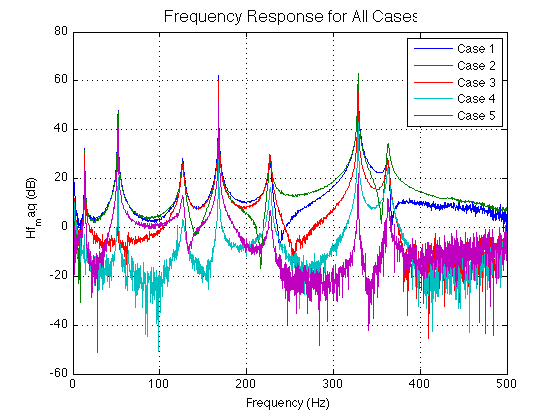
\includegraphics[height = 7.0cm]{Pictures/Lab4_vibes_01.png}
	\caption{\textbf{Frequency Response of Various Excitations.}} 
	\label{fig:cruiseMissile_FRF}
\end{figure}
%
%----------------------------------------------------------------------------------------
%	METHODOLOGY
%----------------------------------------------------------------------------------------
\section*{Methodology}
%
Once the random variables have been defined with appropriate distributions, then FEM's reliability will be evaluated utilizing 5 methods: 
%
\begin{enumerate}
  \item Monte Carlo Sampling (MCS)
  \item First Order Reliability Method (FORM)
  \item Second Order Reliability Method (SORM)
  \item Dimension Reduction Method (DRM)
  \item Sequential Subspace Robustness Assessment (SSRA)
\end{enumerate}
%
The mean and standard deviation of each natural frequency will be evaluated with each method and the number of FE evaluations will be recorded. An empty table can be found in Table \ref{table:METHODS}.
%
\begin{table}[H]
\centering
\caption{\textbf{Reliability Assessment Methods}. This chart will be duplicated for the first 5 natural frequencies.}
\begin{tabular}{| c || c | c | c | c | c |}
\hline
		 & MCS & FORM & SORM  & DRM & SSRA\\ \hline
		\hline
		MEAN  &  -  & -  & - & - & - \\ \hline
		STDEV  &  -  & -  & - & - & -  \\ \hline
		No. of F.E.  &  -  & -  & - & - & -\\ \hline
\end{tabular}
\label{table:METHODS}
\end{table}
% 
After determining the means and standard deviations from each method the MCS will be treated as the true solution. The percent error is calculated by Eq. \ref{eq:error}. The final results will be presented in a table similar to Table \ref{table:ERROR_MCS} for each natural frequency.
%
\begin{gather}
	Error (\%) = \frac{MCS-method}{MCS} \text{x} 100
	\label{eq:error}
\end{gather}
%
\begin{table}[H]
\centering
\caption{\textbf{Error Assessment }. This chart will be duplicated for the first 5 natural frequencies.}
\begin{tabular}{| c || c | c | c | c | c |}
\hline
		 & FORM & SORM  & DRM & SSRA\\ \hline
		\hline
		MEAN   & -  & - & - & - \\ \hline
		STDEV  & -  & - & - & -  \\ \hline
		No. of F.E.  & -  & - & - & -\\ \hline
\end{tabular}
\label{table:ERROR_MCS}
\end{table}

%
%----------------------------------------------------------------------------------------
%	Appendix 1
%----------------------------------------------------------------------------------------
%
%\newpage
%\section*{Appendix 1}



%\newpage

\end{document}